\section{Bayesian Updating}
\label{sec:02_filter}

Assuming gaussian distribution of the single robot results,
the multi-agent decision process is done by Bayesian Updating.
One dimensional probability density functions of states with
variance $\sigma^2$ and mean $\mu$ are described as
\bal
    \mathcal{N}(x,\sigma,\mu) = \frac{1}{\sigma\sqrt{2\pi}}e^{-\frac{(x-\sigma)^2}{2\sigma^2}}.
    \label{eq:02_probabilityDensity}
\eal
Having two values $\mu_0$ and $\mu_1$ with their variances,
the result $\mu'$ of the combination of both is
\bal
    \mathcal{N}(x,\sigma',\mu') = \mathcal{N}(x,\sigma_0',\mu_0') \cdot \mathcal{N}(x,\sigma_1',\mu_1').
    \label{eq:02_newProbabilityDensity}
\eal
By substitution and conversion, $\mu'$ and $\sigma'^2$ can be
formulated to
\bsub
\label{eq:02_intersectionState}
\bal
    \mu' &= \mu_0 + \frac{\sigma_0^2(\mu_1-\mu_0)}{\sigma_0^2+\sigma_1^2}\\
    \sigma'^2 &= \sigma_0^2 - \frac{\sigma_0^4}{\sigma_0^2+\sigma_1^2}.
\eal
\esub

\subsection{Two Dimensional Case}
\label{subsec:02_2dTeam}

Imaging having results from two agents $robot_j$, $robot_k$ that accomplished the \ac{WSDE} algorithm by
computing the \ac{TDOA} with any method, either the \ac{WSDE} angles of both robots
cross and an intersection point would be found or no final whistle source position result arises.
Each of these intersection points $\vec{i_{jk}}$ can be described as whistle source position
state $\vec{\mu_{jk}}$ with variance $\textbit{C}_{jk}$ in accordance to \cref{eq:02_probabilityDensity}.
% -------------------------------------------------------------

Furthermore, the following nomenclature applies:
\begin{itemize}
\item $\vec{v}$: vector pointing at $\left( \begin{matrix} v_x \\ v_y \end{matrix} \right)$ in
      x- and y-coordinates
\item \textbit{M}: matrix with elements $\left( \begin{matrix} m_{xx} & m_{xy} \\ m_{yx} & m_{yy} \end{matrix} \right)$.
\end{itemize}
Final whistle source position $\vec{\mu}$ of all robots is estimated by iterating over
all intersections and updating the result with \cref{eq:02_intersectionState}.

Exemplary, two robots at position $\vec{p_j}$ and $\vec{p_k}$ with their \ac{WSDE} results
are illustrated in \cref{fig:03_rays}.
\begin{figure}[ht]
	\centering
		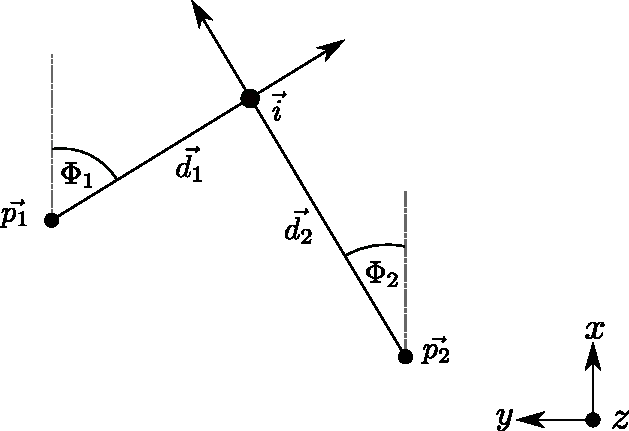
\includegraphics[width=0.50\textwidth]{figures/rays}
    \caption[Nomenclature for multi-agent localization algorithm]
            {Nomenclature for multi-agent localization algorithm.}
    \label{fig:03_rays}
\end{figure}
% -------------------------------------------------------------

Every \ac{WSDE} result is represented as \textit{ray} which consists of the robot position
$\vec{p_j}$ and the \ac{WSDE} angle $\Phi_j$, both in field coordinates.
The \ac{WSDE} angle $\gamma_j$ is defined relative to the robot and the robot's orientation $\theta_j$
is known by its team-message information.
Thus, the absolute angle is
\bal
\Phi_j &= \theta_j + \gamma_j\\
\intertext{from which the whistle source direction ray can be described as}
\vec{r_j} &= \vec{p_j} + \vec{d_j} % = \begin{pmatrix}p_{jx}\\p_{jy}\end{pmatrix} + \ell \begin{pmatrix}d_{jx}\\d_{jy}\end{pmatrix}
    = \begin{pmatrix}p_{jx}\\p_{jy}\end{pmatrix} + \ell \begin{pmatrix}\cos(\Phi_j)\\\sin(\Phi_j)\end{pmatrix}.
\label{eq:03_ray}
\eal

An position of an intersection point by two rays $\vec{r_j}$ and $\vec{r_k}$ is expressed as
\bal
    \vec{\mu_{jk}} &= \begin{pmatrix}\mu_{jkx}\\\mu_{jky}\end{pmatrix}
\eal
with x- and y-coordinates.
If two real numbers $u$ and $v$ exist, so that
\bal
    \vec{\mu_{jk}} &= \vec{p_j} + u \cdot \vec{d_j} = \vec{p_k} + v \cdot \vec{d_k}
    \label{eq:03_intersection}
    \\
    \intertext{a intersection point can be determined by simple geometrical relations.
               With the given terms and conditions $u$ and $v$ values are computed by
               dividing the vectors into x- and y-value and solving the equations, resulting in}
    u &= \frac{p_{jy} \cdot d_{kx} + d_{ky} \cdot p_{kx} - p_{ky} \cdot d_{kx} - d_{ky} \cdot p_{jx}}
            {d_{jx} \cdot d_{ky} - d_{jy} \cdot d_{kx}}
            \label{eq:03_intersectionU}
            \\
    v &= \frac{p_{jx} + d_{jx} \cdot u - p_{kx}}{d_{kx}}.
\eal
% -------------------------------------------------------------

% DEFINITION COVARIANCE MATRIX
The covariance matrix $\textbit{C}_{jk}$ is obtained in the spirit of an Extended Kalman filter \cite{kalman}
considering the Jacobian matrix of an intersection point $\textbit{J}_{i}(\Phi_j, \Phi_k)$ and the average angle error $\varepsilon_{\Phi}$
over all available measurements.
Expressing the direction vector $\vec{d}_j$ of the ray by angle $\Phi_j$ as in \cref{eq:03_ray}, the covariance
matrix of the intersection of two rays $\vec{r}_j$ and $\vec{r}_k$ is
\bsub
\label{eq:03_cov}
\bal
\textbit{C}_{jk} &= \left( \begin{matrix}
                        \varepsilon_{\Phi} & 0 \\
                        0 & \varepsilon_{\Phi} \\
                      \end{matrix} \right) \cdot \textbit{J}_i(\Phi_j, \Phi_k)
     =
    \left(\begin{matrix}
        \sigma_{xx}^2 & 0 \\ 0 & \sigma_{yy}^2 \\
    \end{matrix}\right)
\\
\intertext{with the Jacobian matrix}
\textbit{J}_i(\Phi_j, \Phi_k) &= \left(\begin{matrix}
    \frac{\partial \mu_x}{\partial \Phi_j} & \frac{\partial \mu_x}{\partial \Phi_k} \\
    \frac{\partial \mu_y}{\partial \Phi_j} & \frac{\partial \mu_y}{\partial \Phi_k} \\
    \end{matrix}\right).
\eal
\esub
The elements of the Jacobian result by derivation of the intersection formula \cref{eq:03_intersection}
with \cref{eq:03_intersectionU,eq:03_ray} which yield
\begin{align*}
\frac{\partial \mu_x}{\partial \Phi_j} &= \frac{(\cos(\Phi_k) \cdot (\cos(\Phi_j)^2 + \sin(\Phi_j)^2) \cdot ((p_{jy} - p_{ky}) \cdot \cos(\Phi_k) +
                                  (-p_{jx} + p_{kx}) \cdot \sin(\Phi_k)))}
                                  {(-\cos(\Phi_k) \cdot \sin(\Phi_j) + \cos(\Phi_j) \cdot \sin(\Phi_k))^2}
                                  \\
\frac{\partial \mu_x}{\partial \Phi_k} &= \frac{-(\cos(\Phi_j) \cdot (\cos(\Phi_k)^2 + \sin(\Phi_k)^2) \cdot ((p_{jy} - p_{ky}) \cdot \cos(\Phi_j) + (-p_{jx} + p_{kx}) \cdot \sin(\Phi_j)))}
                                {(\cos(\Phi_j) \cdot \sin(\Phi_k) - \cos(\Phi_k) \cdot \sin(\Phi_j))^2}
                                \\
\frac{\partial \mu_y}{\partial \Phi_j} &= \frac{(\cos(\Phi_j)^2 + \sin(\Phi_j)^2) \cdot \sin(\Phi_k) \cdot ((p_{jy} - p_{ky}) \cdot \cos(\Phi_k) + (-p_{jx} + p_{kx}) \cdot \sin(\Phi_k))}
                                {(-\cos(\Phi_k) \cdot \sin(\Phi_j) + \cos(\Phi_j) \cdot \sin(\Phi_k))^2}
                                \\
\frac{\partial \mu_y}{\partial \Phi_k} &= \frac{(\cos(\Phi_k)^2 + \sin(\Phi_k)^2) \cdot \sin(\Phi_j) \cdot ((-p_{jy} + p_{ky}) \cdot \cos(\Phi_j) + (p_{jx} - p_{kx}) \cdot \sin(\Phi_j))}
                                {(\cos(\Phi_j) \cdot \sin(\Phi_k) - \cos(\Phi_k) \cdot \sin(\Phi_j))^2}.
%  \label{eq:03_jacobianElements}
\end{align*}
% -------------------------------------------------------------

% IN MATRIX FORMULATION
The one-dimensional formulation \cref{eq:02_intersectionState} can be rewritten by defining
an updating matrix \textbit{K} as combination of present and incoming covariance
\bal
    \textbit{K} = \frac{\textbit{C}}{\textbit{C} + \textbit{C}_{jk}}.
\eal

It follows the new two-dimensional probability density function for the estimated
whistle position with
\bsub
\bal
    \vec{\mu}' &= \vec{\mu} + \textbit{K} \cdot \left(\vec{\mu_{jk}} - \vec{\mu}\right)
    \\
    \intertext{being the latest state along with}
    \textbit{C}' &= \textbit{C} = \textbit{C} - \textbit{K} \cdot \textbit{C}
\eal
\esub
as its updated covariance matrix.